\newpage
\section{Extending your transformation}
\genHeader

At this point, we now have a working TGG triple to transform a \texttt{Dictionary} into a \texttt{Box} with three \texttt{partition}s, and a \texttt{Box} with
exactly three \texttt{Partition}s into \texttt{Dictionary}. The only potential problem is that a learning box with only three partitions may not be the most
useful studying tool. After all, the more partitions you have, the more practice you'll have with the cards by being quizzed again and again.

Let's try adding a fourth partition to \texttt{source.xmi} and run the TGG again. Given that we have a rule to transform three partitions, it should at least
complete a partial transformation on them, right? 

\begin{itemize}

\item[$\blacktriangleright$] Add a \texttt{partition3} with one \texttt{card} to your \texttt{source.xmi} so that it resembles
Fig.~\ref{fig:fourthPartitionStart}. Don't forget to set the partition's \texttt{previous} attribute to \texttt{partition0}, and \texttt{partition2.next} to
\texttt{partition3}.

\begin{figure}[htbp]
\begin{center}
  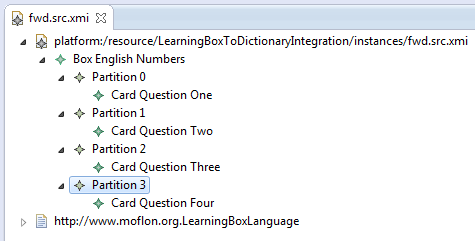
\includegraphics[width=0.7\textwidth]{eclipse_fillFourthPartition}
  \caption{Adding a fourth partition to \texttt{Box}}
  \label{fig:fourthPartitionStart}
\end{center}
\end{figure}

\item[$\blacktriangleright$] An error should appear in the eMolfon console window stating that there was a problem translating your new partition, but the
forward transformation was still able to finish. In fact, if you open \texttt{source.xmi\_FWD.xmi}, you'll be able to confirm the \texttt{English Numbers
Dictionary} was still created and includes your newest card! Let's run the integrator on \texttt{corr\_fwd.xmi} once more to find out exactly how this worked.

\item[$\blacktriangleright$] Start once again with \texttt{Box}, and proceed until the integrator reaches your fourth partition. You'll notice that it
first delays processing the \texttt{partition} as it cannot find a valid rule candidate.\footnote{The message 'Possible Rule Candidate(s): ' will not be
displayed here as the element is simply ignored} Instead, it goes ahead and tries to process \texttt{card}.

\item[$\blacktriangleright$] Here the transformation is able to find a valid rule but opts to delay the action as \texttt{CardToEntryRule} needs the black
\texttt{partition} element from the \texttt{partition} to complete.\footnote{Review the \texttt{source} of your rule if confused}

\item[$\blacktriangleright$] Returning to \texttt{partition}, the transformation detects an endlessly repeating result of not finding a valid rule and so,
terminates the action. Instead of canceling the entire transformation however, it takes an optimistic approach and tries to solve \texttt{Question Four}
\emph{anyway}. The action succeeds!

\begin{figure}[htb]
\begin{center}
  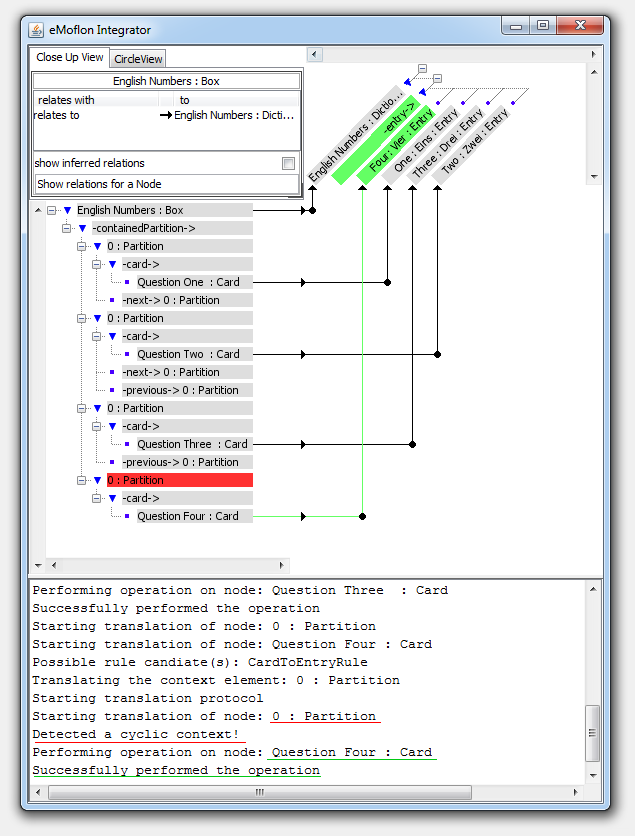
\includegraphics[width=0.7\textwidth]{eclipse_integratorDebug}
  \caption{Detecting errors with the integrator}
  \label{fig:integrator_debugSuccess}
\end{center}
\end{figure}

\item[$\blacktriangleright$] The final task is to try and resolve each of the link variables, but it fails to find rule candidates for any of \texttt{previous},
\texttt{containedPartition}, or \texttt{next}, and so the transformation ends.

\clearpage

We're now presented with a dilemma. This rule, while giving us an error, \emph{works}! Our goal was never the to be able to put an \texttt{Entry} into
partitions with indexes greater than two,\footnote{As resolved in the \texttt{IndexTolevel} implementation} but simply to be able to put any \texttt{card} into
a \texttt{Dictionary}. So why not leave our transformation like this?

\vspace{0.5cm}

In short, it just feels \emph{dirty}. It just cooperates with you and manages to get the job done, and that's it. Instead, let's add a new rule to handle this
additional structure. We could keep things simple by extending the existing \texttt{BoxToDictionaryRule} by connecting a fourth partition, what if we wanted a
fifth one? A sixth? As you can see, this obviously won't work -- there will always be the potential for a \texttt{n+1}th card in an \texttt{n}-sized
box. 

\vspace{0.5cm}

While building this rule, keep in mind that the goal is to simply handle any additional elements and their connecting link variables in \texttt{Box}. This means
we don't need to create any new \emph{correspondence types} to \texttt{Dictionary}.

\end{itemize}

\jumpDual{allCards vis}{allCards tex}


\newpage
\hypertarget{allCards vis}{}
\subsection{AllOtherPartitionsRule}
\genHeader

\begin{itemize}

\item[$\blacktriangleright$] Create a new rule \texttt{AllOtherPartitionsRule}, and complete it according to \Cref{fig:ea_AllOtherPartitionsRuleComplete}.


\begin{figure}[htbp]
\begin{center}
  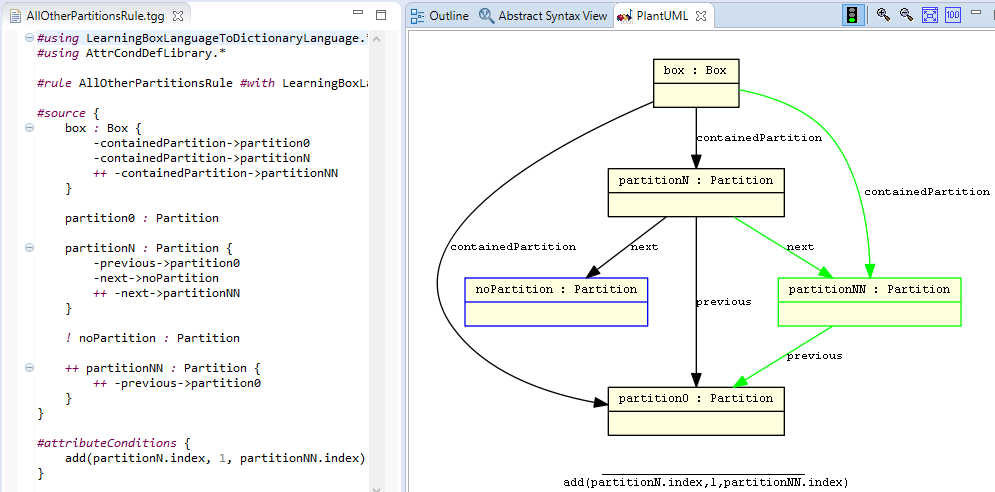
\includegraphics[width=\textwidth]{ea_AllOtherPartitionsRule}
  \caption{The completed \texttt{AllOtherPartitionsRule}}
  \label{fig:ea_AllOtherPartitionsRuleComplete}
\end{center}
\end{figure}

\item[$\blacktriangleright$] As you can see, this rule doesn't assume to know the final \texttt{partition} in the transformation. 
It matches the \texttt{n}th partition as the partition without any next partition, then connects a new \texttt{n+1}th partition to \texttt{n} and \texttt{partition0} (clear as every partitions previous is \texttt{partition0}).
Note that TGG transformations assume that the models are valid, i.e., have the expected structure (in our case meaning that the learning box is correctly ``wired'').\footnote{This should actually be formalised with a set of metamodel constraints that must be checked before a transformation is run, but we've omitted this here to simplify things.}  
Remember that ``blue'' means ``negative''.

\item[$\blacktriangleright$] Generate code for your improved TGG and re-run the transformation. 
It should work now without any error message.
Inspect the protocol to understand what happened.

\item[$\blacktriangleright$] Go ahead and add as many \texttt{partition}s and \texttt{card}s as you like to your model instance.
Your TGG is now also able to handle a \texttt{box} with any number of \texttt{partition}s beautifully.
For five partitions all with cards, the protocol gets quite interesting and is no longer a flat tree.
Try it out! 

\end{itemize}



%%% Local Variables: 
%%% mode: latex
%%% TeX-master: "../src/TGG_mainFile"
%%% End: 


\newpage
\hypertarget{allCards tex}{}
\subsection{AllOtherCardsRule}
\texHeader

\begin{itemize}

\item[$\blacktriangleright$] Right click on the \texttt{rules} folder again and create \texttt{AllOtherCardsRule}. Complete the rule until your file resembles
Fig.~\ref{fig:eclipse_allOtherCardsRule}.

\vspace{0.5cm}

\begin{figure}[htbp]
\begin{center}
  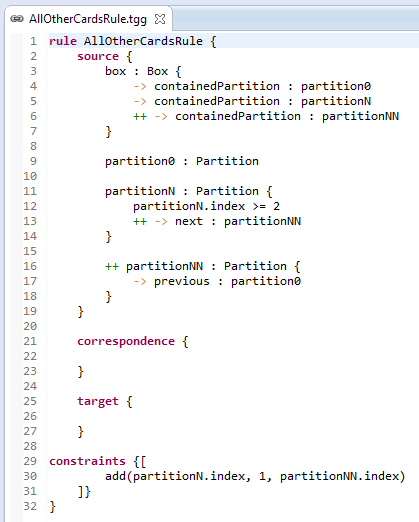
\includegraphics[width=0.7\textwidth]{eclipse_allOtherCardsRule}
  \caption{A complete \texttt{AllOtherCardsRule}}
  \label{fig:eclipse_allOtherCardsRule}
\end{center}
\end{figure}

\item[$\blacktriangleright$] You'll notice that \texttt{box} and \texttt{partition0} have been established as `black' objects -- this rule may only be evaluated
when these objects are already known (and simply need to be adjusted), so we can use their values from the context of the transformation.

\vspace{0.5cm}

\item[$\blacktriangleright$] A second partition, \texttt{partitionN}, has also been established from the context. It represents the \texttt{n}th or last
partition in a \texttt{box} (with an index of 2 or higher), whose \texttt{next} reference will be updated in order to provide an access
link to the newest element, \texttt{partitionNN}.

\newpage

\item[$\blacktriangleright$] Given that the \texttt{add(a,b,c)} syntax is \texttt{a+b=c}, the sole constraint of this rule sets the \texttt{index} of the
\texttt{n+1}th partition so that the \texttt{partition}s are still listed in order.

\vspace{0.5cm}

\item[$\blacktriangleright$] That's it! Save and build your package explorer, then run the TGG again with the `extra' \texttt{partition} to confirm it worked!
You are now free to add as many \texttt{partition}s and \texttt{card}s to \texttt{source.xmi} -- the transformation is now able to elegantly handle them all.

\vspace{0.5cm}

\item[$\blacktriangleright$] Be sure to check out how this rule is implemented in eMoflon's visual specification with Fig.~\ref{fig:ea_allOtherCardsRule} from
the previous section.

\end{itemize}


% Not needed? remind users to check out and read the protocol in their syyntaxes for detail or run the integrator.
% \newpage
\section{The Protocol Explained}
\genHeader

% files are saved and built/refereshed in the Eclipse workspace.

Now that everything is working correctly, let's return to one of the generated protocol files and quickly review what happens in greater detail. Though it looks
scary, this file can prove to be useful if the integrator was ever to fail again, or if you simply wanted to know more detail about what happened during the
transformation process.

\ldots

